% !TEX root = ../my-thesis.tex
%
\chapter{進階動態規劃}
\label{sec:dp2:intro}

\section{章節介紹 Introduction}
動態規劃(Dynamic Programming, 簡稱為DP)是演算法設計中的一個重要概念/方法,雖然它的核心原理並不難,但是狀態的設計千變萬化,往往又能結合其他演算法的概念對轉移做加速,能夠解決五花八門的問題,因此前人對DP這門學問也有不少的研究與探討。
本章節為進階DP,假定讀者對基礎DP、圖論與資料結構已經有一定程度的概念,在基礎DP之上再加上一點小變化,介紹一些跟DP相關、在一般競賽中難度大約屬於中等偏易~中等偏難的技巧。此外,筆者希望藉由挑出一些較具代表性、教育性的問題供讀者思考/欣賞,讓讀者在讀完此篇章節後能對DP這門學問有更加深刻的理解。

本章節會討論的主題大致如下:
\begin{enumerate}
\item DP的理論與設計:此部分算是對基礎DP的複習,主要講DP的理論觀點和證明方法。
\item 常見DP優化:轉移往往是DP解法複雜度的一個瓶頸,本篇章介紹如何使用線段樹、單調佇列等方法加速轉移。
\item 進階DP技巧:羅列一些較困難的經典DP技巧供讀者欣賞與思考。
\end{enumerate}

\section{DP的理論與設計}
\label{sec:dp2:theory}
競賽中解題大多著重直覺,對理論與證明的理解似乎不會對比賽有直接的影響。但筆者認為隨著問題不斷變難,扎實的理論基礎和證明經驗會漸漸變得重要,成為設計新演算法時重要的基石。筆者在此篇希望讓從來沒看過證明的讀者能夠有機會接觸到證明的邏輯,若已熟知證明方法的讀者就稍微忍耐一下,當作複習吧!

\subsection{最佳子結構}
\label{sec:dp2:theory:correctness}
相信大家都知道適合使用DP解決的問題通常會滿足兩大性質:「最佳子結構」(optimal substructure)和「重複子問題」(overlapping sub-problems),其中重複子問題與DP的複雜度比較有關,因此筆者將重心放在與正確性有直接關係的最佳子結構上。

最佳子結構,顧名思義,指的是一個最佳化問題\footnote{最佳化問題(optimization problem), 直覺地講指的就是要找出最大值或最小值的這類問題}的最佳解會被它的子問題的最佳解所決定,相信對基礎DP有所了解的讀者都能夠明白這個描述代表的意義,因此直接看一個簡單的例題,展示證明最佳子結構常見的「交換」手法。

\problembox{最長共同子序列 (LCS)}{經典問題}{
給定兩個字串$A$、$B$,試求$A$與$B$最長共同子序列長度。
}

相信這個問題大家都知道如何解,首先,令$N, M$分別表示$A, B$的長度,$dp(i, j)$令為$A$的後綴$A[i ... N]$與$B$的後綴$B[j ... M]$的最長共同子序列,顯然$dp(1, 1)$即為所求,且$dp(i, j) =
\begin{cases}
0 & \mbox{if } i>N \mbox{ or } j>M\\
dp(i + 1, j + 1) + 1 & \mbox{else if } A[i]=B[j]\\
\max(dp(i + 1, j), dp(i, j + 1)) & \mbox{else if } A[i] \neq B[j]
\end{cases}$
\\
那麼,該如何嚴謹地證明這個轉移式是對的呢?筆者把重點放在第二條式子,若$A[i]=B[j]$,則$dp(i, j)$所代表的最長子序列可以分出三種可能(可能一次符合多種):
\begin{enumerate}
\item $A[i]$沒被使用,沒有出現在最長共同子序列中,此時最佳解為$dp(i + 1, j)$。
\item $B[j]$沒被使用,沒有出現在最長共同子序列中,此時最佳解為$dp(i, j + 1)$。
\item $A[i]$與$B[j]$皆有被使用,皆出現在最長共同子序列中,此時最佳解為$dp(i + 1, j + 1) + 1$。
\end{enumerate}
顯然所有的共同子序列都必須符合至少一種上述情形,若是將三種情況下的最佳解都枚舉到的話必定可以算出$dp(i, j)$。

現在來一條一條分析,若最長共同子序列符合第一種情形,那麼答案必定是$A[(i + 1) ... N]$與$B[j ... M]$的共同子序列,且所有$A[(i+1) ... N]$與$B[j ... M]$的共同子序列都能成為答案的候選,\textbf{在所有候選中,選擇最長的那個共同子序列必定是最好的},要證明這件事通常會使用反證法,假設最佳解符合第一種情形,卻沒有選擇$A[(i+1) ... N]$與$B[j ... M]$的最長共同子序列做為答案,那會發現把它換成最長的選法,會得到一個比最佳解更長且同樣合法的解,這產生了一個矛盾,顯然前提不可能成立。這就是為甚麼在dp轉移中可以宣稱符合第一種情形的最長共同子序列會等於$dp(i + 1, j)$,讀者可以利用相似的論證證明剩下的兩個情形。

那麼,為甚麼在推導出來的三條等式中,可以只選擇$dp(i + 1, j + 1) + 1$作為最終的答案呢?這是因為若$A[i]$與$B[j]$明明可以配對(配對指的是使他們皆出現在所求的最長共同子序列中)卻不配的話,又可以再次把最佳解換掉,而且解必定不會變差。

這可以如此證明:假設沒有任何一種最佳解包含$A[i]$與$B[j]$這組配對,那麼任選一最佳解$S^*$來觀察,若$S^*$中決定將$A[i]$與某個$B[k]$配對,$k \neq j$,此時$B[j]$不可能有配對,因此可以把$A[i]$與$B[k]$拆散,讓$A[i]$去配對$B[j]$,如此一減一增,答案仍跟最佳解一樣好,這得到一個矛盾,除了這個可能以外,其他還有兩種可能\footnote{所有情形有:$A[i]$有配對$B[j]$沒有、$A[i]$沒有配對$B[j]$有、$A[i]$及$B[j]$皆無配對,請讀者自行思考為何只有這三種可能。},亦可用此手法證明,因此必定有一種最佳解選擇$A[i]$與$B[j]$配對的策略,只需枚舉這一種策略就能夠得到最佳解。此種\textbf{「若是最佳解和我的解法策略不同,我必定可以找到一個方法把它的策略換成跟我的一樣,並且保證答案不會變差」}的證明手法在證明DP與greedy的正確性是非常常見的。

\subsection{圖論觀點}
\label{sec:dp2:theory:graph}
學過DP的人肯定聽說過DP與有向無環圖(以下簡稱為DAG)\footnote{directed acyclic graph, 簡稱DAG,指邊有方向性,且圖上不存在任何環的圖}有所關聯,同樣以最長共同子序列當作例子,如果將每個$dp(i, j)$當作圖上一個點,並將$dp(i, j)$連出一條邊指向遞迴式中\textbf{可能}和$dp(i, j)$有關聯的子問題,也就是$dp(i - 1, j), dp(i, j - 1), dp(i - 1, j - 1)$三個點,會得到一張如下的圖:\\
\begin{figure}[h]
	\begin{center}
		\centerline{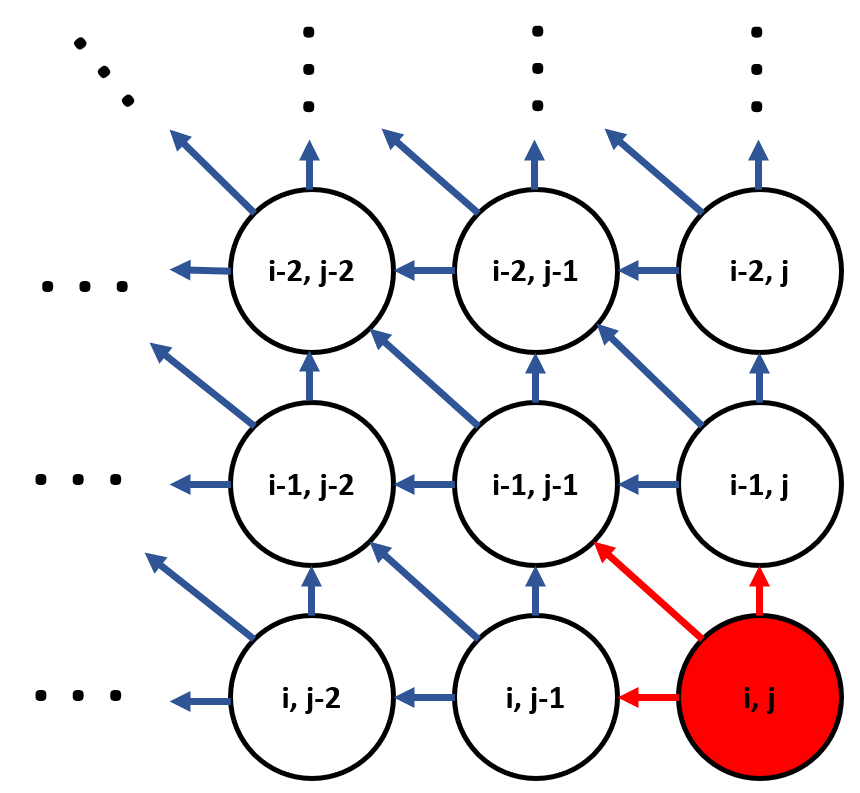
\includegraphics[scale=0.4]{./DP2/LCS_DAG.png}}
		\caption{LCS的轉移,點表示狀態,邊表示此狀態可能參照的子問題,當算到任一點(i,j)時,點(i-1, j-1), (i-1,j), (i, j-1)必須已經被算好可使用,任何滿足此條件的填表順序都可以用來bottom up算DP表}
		\label{figure:dp2:LCS_DAG}
	\end{center}
\end{figure}

很容易看出此圖上邊有方向性,且不存在環,符合有向無環圖的定義,這個性質可以如此證明:由某個點$(i, j)$出發,沿著一條邊走,可能到達的點為$(i - 1, j)$,$(i, j - 1)$,$(i - 1, j - 1)$,無論何種走法,\textbf{走之前與走之後,所在位置的兩座標值加總必定嚴格遞減},更明確地說,座標總和至少減少了$1$,假設圖上存在一環,那想像有一條路徑沿著這個環走一圈,這條路徑由環上某一點,假設為$(x, y)$出發,沿路經過一條以上的邊,最後回到自己,這條路徑起終點同為$(x, y)$,座標值加總相等,這和「每走一步座標值加總至少減$1$」產生了矛盾,因此圖上不可能存在環。

由於這張圖並沒有環,所以有辦法找出一個「好的順序」來計算dp,這個順序必須滿足\textbf{當$(i, j)$要被計算時,所有它指向的子問題都已計算完成},也就是這張圖的任何一組反向拓樸順序(topological order),可以發現平常DP經常使用的row major順序即為其中一種反向拓樸排序。

解DP問題時,只要畫出轉移的關係圖,通常所有計算的順序,以及是否能用滾動數組壓低記憶體等等都可以一目瞭然,因此在比賽時若是遇到題目超出自己能力範圍,心情又很緊張時,不妨靜下心來畫出關係圖,也許就能夠順利解出題目囉。此外,細心的讀者或許會發現,若是建邊時考慮轉移的可能性,並適當地賦予邊權0或1,那麼原問題就變成了這張圖的某種最長路徑問題了,沒錯,DP的解法常常可以視作有向無環圖上的路徑問題,但是人在思考時通常還是由DP、狀態定義與轉移的觀點切入,並非由圖或路徑的觀點切入。

在這節的最後,讀者不妨思考,若是一個問題存在遞迴關係,卻發現畫出的關係圖上有環,那會怎麼樣呢?這好比有兩人A與B,A說:「B你先把你的答案算完,你算完我就可以算我的答案。」,B說:「好,但是在我算我的答案之前,我必須先知道A的答案。」可以想見,\textbf{這兩個人將會互相等待彼此的答案,不管過了多久都不會有人把答案算出來},這個例子可以輕易推廣到環上有多個狀態的情況,
這說明了當關係圖上有環時,無法找到一個好的順序\textbf{直接}計算定義出的函數。但是這並不代表定義出的狀態無解,不過此時往往就需要圖上有其他性質或者使用圖論/代數上更強的方法。此章節的練習題中有一些與圖論相關的例子,若讀者日後因緣際會修習排隊理論這類純理論的數學課程,或許就會有機會見識到聰明的數學家們使用一些精湛的代數方法去解出存在環的遞迴關係式。

\subsection{樹上DP}
\label{sec:dp2:theory:dp_on_tree}
樹,即無向無環連通圖,這種圖上本身就沒有環\footnote{雖說如此,但若DP的關係圖中一條無向邊的兩個方向都同時存在圖中,那就形成了環,但通常這種遞迴關係仍然是能DP解的,馬上就會看到一個例子},若是想計算的DP函數跟樹上一點有關係,這個函數又可以找到和其他點的遞迴關係,可以想見能夠找出好的順序計算它。實際做法通常跟一般DP類似,這裡直接提供一題例題。
\problembox{Subtree}{AtCoder Educational DP contest}{
有一顆$N$個點的樹,你想把每個點塗成白色或者黑色,一種塗色方法合法若且唯若任兩個黑點間都存在一條由黑點組成的路徑,對於每個點$r \in [1, N]$,試求所有合法塗色方法中,$r$被塗成黑色的方法數。由於答案可能很大,請輸出此數模$M$後的結果。
$N \leq 10^5, M \leq 10^9$
}
假設題目並沒有要對所有的點都求一次,而是給定一點$r$,求$r$塗黑的方法數,這個簡化的問題可以怎麼做?若$r$已確定塗黑,可以以$r$為根的觀點審視這棵樹,對於$r$的任一個小孩(child)$v$,可以分出兩個case:
\begin{enumerate}
\item $v$塗白:對於$v$塗白的任何合法解,$v$底下的整棵子樹都必須完全為白色,這是由於$v$的子孫們到$r$的唯一simple path必須經過$v$,而這條路由於$v$塗白而斷掉了。
\item $v$塗黑:仔細觀察可以發現\textbf{$v$的小孩的處境跟$v$事實上非常相近},能找到遞迴關係。
\end{enumerate}
仔細想一下應可定出如下的狀態,令$dp[v] = $已知$v$的父親(father / parent)被塗成黑色的情況下,有多少方法將$v$底下的子樹合法地著色(合法代表$v$的子樹內任一點都可沿著黑點走回$v$的父親),稍微推導一下可得:

\begin{tabular}{rl}
$dp[v]$&$=$ ($v$塗白色的方法) + ($v$塗黑色的方法) \\
      & $= 1 + \prod_{i=1}^{deg(v)}{dp[c_i]}$, 其中$deg(v)$代表$v$的degree, $c_i$代表$v$的第$i$個小孩。
\end{tabular}


所求 $= \prod_{i=1}^{deg(r)}{dp[c_i]}$ (邊界條件請自行推導)

在這個遞迴式中每個點只要求自己的子孫先把答案算好,明顯是個DAG,通常會選擇DFS的順序去填表(或說post-order traversal的順序,因為$v$的小孩們都算完$dp$後,$v$就可以算出自己的$dp$)。但是原題目對所有的$r$都要求一次,若是枚舉所有點當根重算就需要$\Ord(N^2)$的時間,那該怎麼辦呢?

再觀察一下,會發現一個點$r$的答案需要\textbf{周圍所有點把它成父親的$dp$},如果任選一點$r$當根,除了$r$以外的其他點,都只缺少了「頭上那棵子樹」的方法數,因此可以試著在已知所有$dp[v]$的情況下將它算出來,令$p=$ $r$為根時$v$的父親,$up\_dp[v] =$當$v$為$p$的父親,且$v$為黑色時,$p$所管理的的子樹的合法著色方法。易得$up\_dp[v] = 1 + up\_dp[p] \times \prod_{\{c\mbox{ is child of }p \mbox{ and } c \neq v \}}{dp[c]}$,此處$child$指的是$r$當根下的觀點。
\begin{figure}[ht]
	\begin{center}
		\centerline{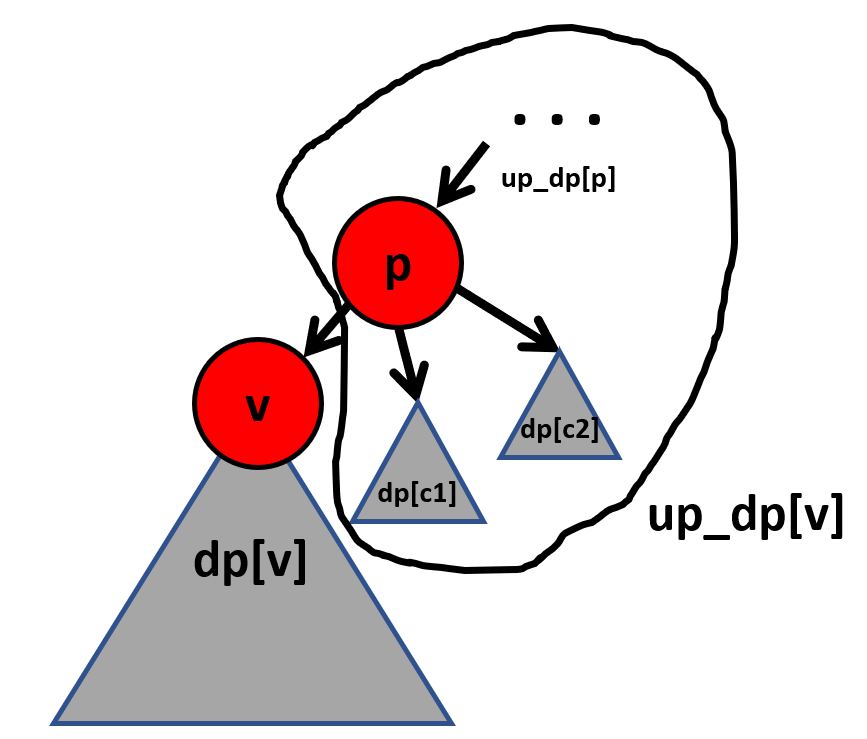
\includegraphics[scale=0.4]{./DP2/dp_on_tree.png}}
		\caption{示意圖,三角形代表子樹,$up\_dp[v]$求將框住的部分視為$v$其中一棵子樹時的方法數}
	\end{center}
\end{figure}
\\
顯然只要有$dp$及$up\_dp$兩個函數,答案就可以輕鬆地求出來,但是直接計算上面的式子將使每個點需要$\Ord{(N)}$的時間,總時間$\Ord(N^2)$,並沒有比直接枚舉所有點當根重算好,不過注意到$p$的所有小孩的轉移非常相似(其實就只是從所有它的小孩們的乘積裡挑掉一點$v$),此方法明顯有地方可以改進,優化的方式及程式碼留待下一章節再做討論。

稍微回顧一下剛才的兩個$dp$總共定了多少狀態呢?向下的$dp$的數量剛好等於樹上邊數,向上的$up\_dp$由於在根節點$r$沒有定義,因此有$N-1$這麼多個,剛好也等於邊數,這個結果並不是巧合。可以想像一下要計算一點$v$的答案時,需要的是由$v$為父親,往周邊的子樹的$dp$,\textbf{所有需要的$dp$聯集起來,就像是對於每條無向的邊$(u, v)$,都需要它兩種不同方向$(u, v)$以及$(v, u)$的$dp$},因此,這種「計算我頭上的那棵子樹的答案」的DP也可看成在計算「每條邊兩個方向分別的DP」,而上述的解法有點像是取一個基準點$r$,將一棵無向的樹拆分成兩個DAG,分別求取DAG上的邊的DP值\footnote{這個說法並沒有非常嚴謹,因為許多無向圖,例如一個簡單環,都有辦法將拆成兩個DAG的聯集,但是定義在圖上的DP卻未必可行,筆者也不確定是否只有樹能這麼做}。

值得一提的是,由於樹上任兩點只有唯一的simple path,單看一次DFS根本不會有狀態被用到多於一次,因此此問題並沒有重複子問題的性質,也就是說,DP解跟直接遞迴具有完全一樣的複雜度,與其說是DP不如說更像分治,但習慣上還是會稱此種技巧為樹上DP,樹分治指的則是某個更加困難的技巧。不過在這題中,由於算出的每個點的$dp[v]$在日後算答案時都會用到,不得不將整個過程存下來。但是確實許多只關心根節點答案的DP,例如計算有根樹的樹高,是完全沒有重複子問題性質的。

\subsection{練習題}
\label{sec:dp2:theory:exercise}
標示$Hint$的地方可能會毀掉解題的樂趣,建議真的解不出來再去看。
\problembox{Removal Game}{ECNA 2016}{
在一個首尾相接的環上寫著$N$個數字,現在你想不斷把數字從環上移除,每移除一個數字就必須付出目標數字當下左右相鄰數字的GCD,直到剩下兩個數字為止,總花費為中途操作花費加總再加上最後剩下兩個數字的GCD,求最小花費,$N \leq 100$。\newline
$Hint:$ 雖然DP的參數在轉移時看似沒有明顯遞增遞減的項,但轉移很明顯是DAG,確實有某項東西不斷在遞減,填表時未必需要將陣列展開成兩倍。
}
\problembox{最短共同非子序列}{AIZU 1392}{
給定兩個由0與1組成的字串$A$、$B$,試構造一個由0與1組成的字串$S$,使得$S$既非$A$的子序列也非$B$的子序列,且$S$的長度必須是所有合法解中最短的,若有多組解則輸出字典序最小者。$\left|A\right|, \left|B\right| \leq 4000$ \newline
$Hint:$ 若由圖的觀點來看,定義出的DP是在求關係圖上的哪個圖論經典問題?此時DP解和圖論經典演算法解的複雜度相同嗎?
}
\problembox{Special Judge}{TIOJ 2070}{
給你由小寫英文字母組成的字串$X$,請判斷是不是每一個前$K$個英文字母的子集的排列都是$X$的子序列。$\left|X\right| \leq 1000, K \leq 20$ \newline
$Hint:$ 請思考判斷一個字串$T$是否為字串$S$的子序列的過程。
}
\problembox{Undecodable Code}{Live Archive 2475}{
題目敘述較複雜,請在Live Archive上看原題目。\newline
$Hint:$ 雖然是ICPC World Final的題目,但這題概念並不難,試著思考\textbf{「構造一份undecodable code的過程」}該如何用狀態完整描述,列出轉移後,遞迴的關係圖上有環嗎?
}
\problembox{Addition on Segments}{CF 981E}{
題目敘述較複雜,請在Live Archive上看原題目。\newline
$Hint:$ 將DP狀態訂為「可不可以做到」這種0與1的函數往往難以找到遞迴關係,但若是改成「組合出$x$的方法數有幾種」這種比0與1「更困難」的狀態,這個$dp$能夠轉移嗎? (先不考慮方法數可能過大的問題,此外,這題也有資料結構解)
}
\problembox{Three Religions}{CF 1149B}{
題目敘述較複雜,請在Codeforces上看原題目。\newline
$Hint:$ 試著列出一個三維的DP, 當發生修改時,有多少狀態需要重算?
}
\problembox{Museums Tour}{CF 1137C}{
題目敘述較複雜,請在Codeforces上看原題目。\newline
$Hint:$ 到處都是環,沒有一個順序去計算DP。但其實圖中隱藏著順序,只是直接看看不出來,讀者有學過哪個跟DAG關聯很深的經典演算法 / 經典圖論觀點嗎?
}

\section{常見DP優化}
使用DP解決問題常常會遭遇複雜度太高的問題,此時有兩個大方向,一個是「減少狀態數」,另一個是「優化轉移」,但是一個狀態必須能夠完整表達DP的過程,狀態數不是說減少就能減少,通常需要問題本身有好的性質才能減少。相較之下,優化轉移則有許多標準招數,在本章節中筆者會介紹幾種常見的優化轉移的方法。但是希望讀者能記住,這些技巧只是DP優化的冰山一角,最棒的解法往往是用盡問題的一切特殊性質,而不是套上一些通用的技巧,實際的優化方法千變萬化,有時只需要對問題的一點細心觀察就能得到很好的結果,因此在思考題目時,千萬不要被這些技巧侷限住了。

\subsection{記錄前綴和}
記錄前綴和可說是最簡單的優化方法,簡而言之就是\textbf{觀察不同狀態間轉移的相似之處,並將重複計算的部分記錄下來},也可以說是將每次轉移當成一次區間求和問題,來看看剛才樹DP時用到的例子。

\problembox{Subtree}{AtCoder Educational DP contest}{
有一顆$N$個點的樹,現在你想把每個點塗成白色或者黑色,一種塗色方法合法若且唯若任兩個黑點間都存在一條由黑點組成的路徑,對於每個點$r \in [1, N]$,試求所有合法塗色方法中,$r$被塗成黑色的方法數。由於答案可能很大,請輸出此數模$M$後的結果。
$N \leq 10^5, M \leq 10^9$
}
上一節的討論中已推導出兩個有用的函數$dp[v]$與$up\_dp[v]$,已知$dp[v]$可DFS輕易求出,且有$up\_dp[v] = 1 + up\_dp[p] \times \prod{\{dp[c] : c\mbox{ is child of }p \mbox{ and } c \neq v \}}$,該如何快速求出$up\_dp[v]$呢?上一節已說過,\textbf{對於同一點$p$,他的小孩們需要的轉移非常相似,事實上$p$的任一個小孩$v$需要的值只是$p$所有小孩的$dp$乘積,但是多一個條件:去掉$v$本身。}很直覺會想把每個點小孩的$dp$乘積紀錄下來,想要去掉一點$v$只要把乘積除以$dp[v]$就完成了,但是在題目條件下,未必能在模任意的$M$下做除法(模$M$下的乘法反元素未必存在),所以可以換個方式:假如把$p$的小孩按照任意一個順序排好,給它們編號$c_1, c_2, c_3, ..., c_k, k = deg(p)$,那某個小孩$c_i$要算的值就是將他前面所有人乘起來,再將它後面所有人乘起來,只要改成紀錄前綴乘積與後綴乘積即可達到要求。

由於所有$deg(p)$加起來等於把每條邊算到正好兩次,這些前綴積總共只需要$\Ord(N)$的時間就可以建出來。有了這些前綴積後所有轉移皆為$\Ord(1)$,就可在$\Ord(N)$的時間內解決此問題。

回顧一下這個做法,讀者可能會覺得此題出題者很無聊,刻意卡掉乘法反元素的解法,不然根本不需要紀錄這些前綴積,但是請思考一下,若今天轉移函數為某些子樹中取$max$這類不存在$\Ord(1)$反操作的函數\footnote{事實上,在這題中乘法反元素也無法$\Ord(1)$求出。},那麼這種記錄前綴後綴的技巧就相當有用了!這裡附上此題的程式碼:

\begin{lstlisting}[caption=Subtree的程式碼]

/* G: adjacency list, par[v]: 以1為根時,點v的父親 */
int N, par[MAXN];
LL MOD, dp[MAXN], up_dp[MAXN];
vector<int> G[MAXN];

void dfs1(int v, int p) {
	/* 第一次dfs, 目標是把dp和par算出來, v代表當前點, p代表父親。 */
	par[v] = p;
	dp[v] = 1;

	/* 算v點塗黑的方法,就是找到所有的小孩並遞迴 */
	for (int to : G[v]) {
		if (to != p) {
			dfs1(to, v);
			dp[v] = dp[v] * dp[to] % MOD;
		}
	}

	/* 把整棵樹塗白的方法加進去 */
	dp[v]++;
}

void dfs2(int v, int p) {
	/* 建造前綴積(prefix product), 以開區間實作 */
	LL suff;
	vector<LL> pref(G[v].size() + 1);
	pref[0] = suff = 1;
	for (int i = 0; i < G[v].size(); i++) {
		/* 建造時需特別注意adjacency list中存有v的父親。 */
		LL mul = (G[v][i] == p ? 1 : dp[G[v][i]]);
		pref[i + 1] = pref[i] * mul % MOD;
	}

	/* 後綴積(suffix product)在過程遍歷小孩的過程中維護 */
	for (int i = G[v].size() - 1; i >= 0; i--) {
		if (G[v][i] != p) {
			up_dp[G[v][i]] = (suff * pref[i] % MOD * up_dp[v] + 1)% MOD;
			suff = suff * dp[G[v][i]] % MOD;
			dfs2(G[v][i], v);
		}
	}
}

int main() {
	ios_base::sync_with_stdio(0); cin.tie(0);

	/* 輸入邊,存進G這個adjacency list裡面 */
	cin >> N >> MOD;
	for (int i = 0; i < N - 1; i++) {
		int x, y;
		cin >> x >> y;
		G[x].push_back(y);
		G[y].push_back(x);
	}

	/* 計算主體就是兩次DFS,第一次算dp,第二次算up_dp */
	dfs1(1, 1);
	up_dp[1] = 1;
	dfs2(1, 1);

	/* 建造答案: 將v周圍向外方向的邊乘起來 */
	for (int i = 1; i <= N; i++) {
		LL ans = up_dp[i];
		for (int to : G[i]) {
			if (to != par[i]) {
				ans = ans * dp[to] % MOD;
			}
		}
		cout << ans << "\n";
	}

	return 0;
}
\end{lstlisting}

請注意前綴和的使用時機和方式還有很多很多,雖然此題需要前綴和後綴,但有時只需維護一個總和,又有時要維護多個。不過這些方法的精神都差不多:觀察轉移時的相似之處,想辦法把重複計算的部分紀錄下來而不是每次重算,因此筆者這裡不再多談。

\subsection{配合線段樹}
有時各種狀態的轉移雖然有相似性,但是在DP過程中需要的值需要做一些動態的改變,這時難以修改的前綴和 / 前綴最大值等等存法就不太適合,這時可以改成使用線段樹來做動態的變化,此節中筆者假定讀者已熟習線段樹的各種操作,如$\Ord{(\log N)}$區間求和,區間求最大值,區間同加一值$x$等操作。以下直接用例題展示如何使用線段樹加速轉移。

\problembox{Flowers}{AtCoder Educational DP Contest}{
有$N$朵花排成一列,第$i$朵花的美麗度是$a_i$,高度是$h_i$,現在你想選出一些花,使得被選中的花由左至右高度嚴格遞增,請找出此條件下,選出的花美麗度總和最大的選法。
$N \leq 10^5, 1 \leq a_i \leq 10^9$, $1 \leq a_i \leq N$,所有$h[i]$皆相異。
}
稍微思考一下應該可看出這是最長遞增子序列的變形,只是改
成要最大化被選中者的權重和,可以回想一下最基本的DP解法。令$dp[i] = $以$h_i$為結尾的最大權重(美麗度)遞增子序列,枚舉有機會接在$h_i$前面的所有人,找出其中最好的方案,也就是$dp[i] = \max\{dp[j] : h[j] < h[i], j < i\} + a[i]$。

仔細觀察這個式子,$j < i$這個條件讓整個式子很像是個對$j \in [1, i - 1]$這個範圍的$dp[j]$求取最大值,直覺上會想把所有有興趣的$dp[j]$塞進樹裡求最大值,但是$h[j] < h[i]$卻讓人不知從何下手。這裡可以轉換一下思考方式,同樣以$i$遞增的順序計算DP,並且\textbf{根據高度值決定$dp[i]$在線段樹中的位置},也就是將$dp[i]$放在線段樹中$h[i]$的位置,會發現\textbf{當計算到$i$時,所有 $\geq i$ 的$dp[j]$根本還沒放進樹裡},只要將樹中沒有人被佔據的位置設為$0$,就可發現所求為樹中$[1, h[i] - 1]$的範圍中的最大值,簡記為$RMQ(1, h[i] - 1)$。如此即可在$\Ord (N\log N)$的時間內解決問題。

稍微回顧一下這個演算法,$dp[i]$想枚舉的所有$dp[j]$有兩個範圍上的限制,為了\textbf{正好枚舉到想枚舉的範圍},這個線段樹的做法就像是\textbf{用時間順序解決其中一個範圍限制,並用資料結構的詢問範圍來解決第二個限制},由這個例子應該可以感覺到\textbf{計算順序是非常重要的},事實上決定計算順序往往也是設計演算法的一環,好的計算順序使轉移的性質更能夠被利用,因此希望讀者在實作DP時盡量選擇bottom up的方式,熟悉計算順序的思考
。在這題的最後,希望讀者能夠想想幾個問題,以下問題請注意答案可能不唯一:
\begin{enumerate}
\item 為何在此處把不存在的轉移設為$0$不會造成答案太大或太小? 如果$a[i]$中有負的,轉移時需要做甚麼改變?
\item 如果不同的兩朵花可以有相同高度,線段樹的操作需要做哪些改變?
\item 當所有樹中$[1, h[i] - 1]$的位置都已存在轉移,此作法有枚舉到邊界條件,也就是$a[i]$前面不放任何數字嗎? 如果沒有的話,這個方法還是對的嗎?
\item 當$h[i]$的範圍高達$10^9$,或者可以有負的值,根本放不進樹中,還能套用一樣的演算法嗎?該如何改才能使這個演算法正確運作?
\item 這個作法用時間順序解決$j < i$這個條件,用RMQ的範圍解決$h[j] < h[i]$這個條件,那麼對稱地,可以讓這兩個技巧解決的條件反過來嗎? 如果想用時間順序解決$h[j] < h[i]$這個條件,應該以甚麼樣的順序計算DP才可使\textbf{算到$dp[i]$時,已進到樹中的轉移$dp[j]$皆滿足$h[j] < h[i]$}?
\item 這個演算法每次詢問最大值的範圍總是$dp$這個陣列的前綴,可以改用專門處理前綴的Binary Indexed Tree / Fenwick Tree來解決此問題嗎? 在甚麼情況下可以用Binary Indexed Tree來維護最大值? ($Hint:$ BIT和線段樹都可視作一種將區間切塊的方法,但是BIT中一個區間未必能找到常數個子區間組合而成,因此紀錄的值無法像線段樹那般輕易地bottom up更新)
\end{enumerate}
此處提供使用Binary Indexed Tree的程式碼實作,請注意由於所有$h[i]$皆相異,可以將查詢範圍改成$[1, h[i]]$。
\begin{lstlisting}[caption=使用Binary Indexed Tree解Flower]
struct BIT {
	LL c[MAXN];
	void set(int pos, LL v) {
		/* 將樹的第pos個位置改成v */
		while (pos < MAXN) {
			c[pos] = max(c[pos], v);
			pos += pos & -pos;
		}
	}
	LL RMQ(int pos) {
		/* 查詢樹中[1, pos]的最大值 */
		LL res = 0;
		while (p) {
			res = max(res, c[pos]);
			pos -= pos & -pos;
		}
		return res;
	}
} tree;

int N, h[MAXN], a[MAXN];

int main() {
	ios_base::sync_with_stdio(0);
	cin.tie(0);

	cin >> N;
	for (int i = 1; i <= N; i++) cin >> h[i];
	for (int i = 1; i <= N; i++) cin >> a[i];
	for (int i = 1; i <= N; i++) tree.set(h[i], tree.RMQ(h[i]) + a[i]);

	cout << tree.RMQ(N) << "\n";
}
\end{lstlisting}

接著再看一題較困難的例題。

\problembox{Many Moves}{AtCoder Regular Contest 073}{
有兩個棋子擺在一個$1 \times N$的棋盤上,一個開始一個在位置$A$,另一個則在位置$B$,接下來有$Q$筆指令,第$i$筆指令要求將其中一個棋子移動到$x_i$的位置,\textbf{指令只指定位置,要移動哪一個棋子皆可,並且每次指令你除了將一個棋子移動到$x_i$外不能做其他任何事},將棋子由$s$移動$t$需要花費$\left|s-t\right|$秒,兩個棋子可以同時站在同一格,請問執行完所有指令最少需要多少時間?
$N \leq 10^5, Q \leq 10^5, 1 \leq A, B, x_i \leq N$
}
狀態設計並不是本節的重點,請讀者嘗試自行思考。
觀察到「執行第$i$筆指令時,其中一枚棋子必定在$x[i - 1]$的位置」這個性質後,可以令$dp[i][j] = $將前$i$筆指令執行完成,並使第$i$次指令被操作的那個棋子位置在$x[i]$,另一個沒被動到的棋子位置在$j$的最小花費,轉移時,可以枚舉做完$i-1$筆指令,且沒被動到的棋子在$k$,另一個停在$x[i - 1]$的情況,並考慮要把哪一個棋子移動到$x[i]$,因此有:\\ \\
$dp[i][j] =
\begin{cases}
dp[i - 1][j] + \left|x[i] - x[i - 1]\right|  \mbox{, if } j \neq x[i - 1]\\ \\
\min(dp[i - 1][j] + \left|x[i] - x[i - 1]\right|, \\ \min\{dp[i - 1][k] + \left|x[i] - k\right| : k \in [1, N]\}) \mbox{, if } j = x[i - 1]
\end{cases}$

可發現$j = x[i - 1]$的情況兩項其實重複枚舉了,但為了強調$j = x[i - 1]$的情況轉移其實完全包含$j \neq x[i - 1]$的情況,筆者並沒有將它化簡。想像這個式子想做的事,會發現從$dp[i - 1]$轉移到$dp[i]$時,每個位置都要加上一值$\left|x[i] - x[i - 1]\right|$,並且有一個位置$j = x[i - 1]$需要特別對一個範圍取min。把整個資料結構中所有人同時加值是非常簡單的,只要用一個變數紀錄全部總共加的值$add$,在取用資料結構中的數字時,記得加上同加的值$add$即可,因此以下將重點放在$j = x[i - 1]$時的枚舉範圍上。

首先這個轉移式跟前面直接對某個範圍的$dp$直接求極值不大一樣,但是讀者應該能直覺感受到,當枚舉$k = j - 1$時,需要額外加入花費$1$,枚舉$k = j - 2$時,需要額外加入花費$2$...依此類推,感覺上就是可以維護的!只要透過每個$k$都同減自己的位置$k$,再把結果加上$j$,不就可以達到想要的效果了嗎?有了這個直覺就可以來推導數學式了,首先將絕對值展開,再把與枚舉$k$無關的項提出去。

\begin{tabular}{rl}
所求&$ = \min\{dp[i - 1][k] + \left|x[i] - k\right| : k \in [1, N]\}$ \\ \\
    &$ = \min\{dp[i - 1][k] + x[i] - k : k \in [1, x[i]\}$及 \\
    &$\min\{dp[i - 1][k] - x[i] + k : k \in [x[i], N]\}$兩者取較小值 \\ \\
    &$ = \min\{dp[i - 1][k] - k : k \in [1, x[i]\} + x[i]$及 \\
    &$\min\{dp[i - 1][k] + k : k \in [x[i], N]\} - x[i]$兩者取較小值 \\
\end{tabular}

由此可知,真正想最小化的其實是$dp[i - 1][k] - k$及$dp[i - 1][k] + k$這兩項,與直覺相當吻合,只要兩棵線段樹即可完成所有操作。時間複雜度如下: \newline
\hspace*{1cm} - 建造兩棵線段樹的時間為$\Ord(N)$ \newline
\hspace*{1cm} - 總共有$Q$次指令,每個指令中作:\newline
\hspace*{2cm} - 樹中所有值同加一數: $\Ord(1)$\newline
\hspace*{2cm} - 兩棵樹分別RMQ: \hspace*{0.6cm}$\Ord(\log N)$\newline
\hspace*{2cm} - 兩棵樹分別單點修改: $\Ord(\log N)$\newline \newline
因此這個做法在$\Ord(N + Q\log N)$時間內即可解出此題。

在此節的最後,希望讀者可以注意到幾件事:
\begin{enumerate}
\item 此題的解題過程中把樹中紀錄的值由$dp[j]$改成$dp[j] - j$,那麼在$j \neq x[i - 1]$情形下的線段樹加值操作需要有所改變嗎?為甚麼?
\item 為何狀態定義要強調其中一個棋子是「在第$i$次操作被移動到$x[i]$」,停在$j$的棋子則是「在此次操作沒被動到」這兩個身分?如果定義改成「做完$i$次操作後,其中一個棋子位置在$x[i]$, 另一個位置在$j$」,而不包含任何身分,那麼應該枚舉多少種case才能包含所有可能?將得出的轉移盡可能化簡後,兩種狀態定義下需要枚舉的式子一樣嗎?
\item 這個$dp[i][j]$總共有$\Ord(QN)$個狀態,但是由於轉移實在非常規律,此作法只花了$\Ord(N + Q \log N)$,就把$\Ord(QN)$個狀態全部算完了,也就說,在僅僅$\Ord(N + Q\log N)$的計算過程中,所有$\Ord(QN)$個狀態都曾以直接或不直接的形式出現在記憶體中,相當神奇。
\end{enumerate}

附上程式碼。
\begin{lstlisting}[caption=Many Moves的程式碼]
struct Segment_tree {
	LL add, minv[4*MAXN];

	/* 下面的函式中, l, r, idx都只是記錄線段樹遞迴過程的變數 */
	void init(int l, int r, int idx) {
		/* 初始化,所有狀態皆不存在 */
		add = 0;
		minv[idx] = INF;
		if (l == r) return;
		int m = (l + r) >> 1;
		init(l, m, idx << 1);
		init(m + 1, r, idx << 1 | 1);
	}
	LL universal_add(LL num) {
		/* 整棵樹每個點全部增加num */
		add += num;
	}
	void take_min(int pos, LL val, int l, int r, int idx) {
		/* pos這一點與val取較小值 */
		if (l == r) {
			if (val < minv[idx] + add) {
				minv[idx] = val - add;
			}
			return;
		}
		int m = (l + r) >> 1;
		if (pos <= m) take_min(pos, val, l, m, idx << 1);
		else take_min(pos, val, m + 1, r, idx << 1 | 1);
		minv[idx] = min(minv[idx << 1], minv[idx << 1 | 1]);
	}
	LL RMQ(int ql, int qr, int l, int r, int idx) {
		/* 詢問範圍為ql與qr,求最小值 */
		if (ql <= l && r <= qr) return minv[idx] + add;
		int m = (l + r) >> 1;
		LL res = INF;
		if (ql <= m) res = min(res, RMQ(ql, qr, l, m, idx << 1));
		if (qr >  m) res = min(res, RMQ(ql, qr, m + 1, r, idx << 1 | 1));
		return res;
	}
} tree1, tree2;

int N, Q, A, B, X[MAXN];

int main() {
	ios_base::sync_with_stdio(0); cin.tie(0);

	cin >> N >> Q >> A >> B;

	/* 令x[0] = A, 除了dp[0][B]外的狀態皆不存在 */
	X[0] = A;
	for (int i = 1; i <= Q; i++) {
		cin >> X[i];
	}

	/* 初始化,INF(無限大)代表不存在,dp[0][B]一開始cost為0, 初始值就是0-B與0+B */
	tree1.init(1, N, 1);
	tree2.init(1, N, 1);
	tree1.take_min(B, -B, 1, N, 1);
	tree2.take_min(B, B, 1, N, 1);

	/* DP過程就是全部加值,只有j = x[i - 1]多出一種轉移 */
	for (int i = 1; i <= Q; i++) {
		LL cost = abs(X[i] - X[i - 1]);
		LL result = min(tree1.RMQ(1, X[i], 1, N, 1) + X[i], tree2.RMQ(X[i], N, 1, N, 1) - X[i]);
		tree1.universal_add(cost);
		tree2.universal_add(cost);
		tree1.take_min(X[i - 1], result - X[i - 1], 1, N, 1);
		tree2.take_min(X[i - 1], result + X[i - 1], 1, N, 1);
	}

	/* 由dp[Q][i] - i還原出dp[Q][i] */
	LL ans = INF;
	for (int i = 1; i <= N; i++) {
		ans = min(ans, tree1.RMQ(i, i, 1, N, 1) + i);
	}

	cout << ans << '\n';
}
\end{lstlisting}

\subsection{使用單調佇列}
單調佇列(monotonous queue)是個簡單好用的資料結構,使用在DP時,他的基本精神就是把「適用範圍較小,值又較差」的轉移挑掉,會發現在許多問題中,僅僅是把這些明顯沒用的轉移挑掉,就可以大幅降低搜索最佳轉移的難度。用說的實在有點抽象,直接來看一個例子。

\problembox{Flowers}{AtCoder Educational DP Contest}{
有$N$朵花排成一列,第$i$朵花的美麗度是$a_i$,高度是$h_i$,現在你想選出一些花,使得被選中的花由左至右高度嚴格遞增,請找出此條件下,選出的花美麗度總和最大的選法。
$N \leq 10^5, 1 \leq a_i \leq 10^9$, $1 \leq a_i \leq N$,所有$h[i]$皆相異。
}

沒錯,和前面線段樹DP時一模一樣的題目,回想$dp[i] = \max\{dp[j] : j < i, h[j] < h[i]\} + a[i]$這個DP,假如把每個$j < i$打包成一個$(h[j], dp[j])$的數對,會發現:
\begin{enumerate}
\item $h[j]$就像是「使用這個轉移需要的門檻」,越大越難以使用,嚴謹地描述,就是一個狀態\textbf{在轉移時若能使用較大的$h[j]$,必定也能使用所有較小的$h[j]$},所以$h[j]$應該越小越好。
\item $dp[j]$是價值應該越大越好。
\item 當$i$增加時,可使用的數對只會越來越多,原本可使用的不會被刪減。
\end{enumerate}

因此,對任意一個$(h[j], dp[j])$,若是存在任何一個$(h[k], dp[k])$滿足「使用範圍更廣,價值還更大」,即$h[k] \leq h[j]$且$dp[k] \geq dp[j]$,那麼在往後$(h[j], dp[j])$都不可能成為最佳轉移,可以直接把它扔了。這個想法雖然看起來不過像是個平凡的常數優化,但這一扔不得了,可以發現扔完後剩下的轉移中,\textbf{當門檻,也就是$h[j]$增加時,$dp[j]$勢必要跟著增加,否則就與上述的規則衝突}。

此時若想在維護好的數對$(h[j], d[j])$中找出$h[i]$可用的最佳轉移時,\textbf{只要搜出所有$h[j]$中最後一個$< h[i]$的就是最佳轉移了,假設這些數對已經依照$h[j]$排好,這變成是一次二分搜索就可解決的問題!},現在只要把所有轉移按照$h[j]$排好,並在有新的$(h[k], dp[k])$加進來時好好維護資料結構就行了,實作上可使用二分搜索樹來維護排好的$h[j]$序列。這種維護一些數對,使得它們兩個維度總是同時嚴格增 / 減的資料結構就稱為單調佇列。以下提供程式碼供讀者思考。

\begin{lstlisting}[caption=Flowers的程式碼2]
int N, h[MAXN], a[MAXN];
LL dp[MAXN];
set<int> mque;

int main() {
	ios_base::sync_with_stdio(0); cin.tie(0);

	cin >> N;
	for (int i = 1; i <= N; i++) cin >> h[i];
	for (int i = 1; i <= N; i++) cin >> a[h[i]];

	/* mque即單調佇列,這題有h[i]互相不同又<=N的條件,只要知道h[i]立刻可以拿到dp[i],不需要真的存數對。 */
	mque.insert(0);
	for (int i = 1; i <= N; i++) {
		/* 假設結構已經維護好,只要二分搜索找到最後一個能用的即可 */
		auto it = mque.upper_bound(h[i]);
		dp[h[i]] = dp[*prev(it)] + a[h[i]];

		/* 將(h[i], dp[i])放入結構中,其中h[j] <= h[i]者因為適用範圍較廣,不可能因為h[i]而被拿掉,剩下哪些人該拿掉由讀者自行思考,尤其注意為何h[i]必定可以進入mque中 */
		while (it != mque.end() && dp[h[i]] >= dp[*it]) {
		    it = mque.erase(it);
		}
		mque.insert(h[i]);
	}

	cout << dp[*mque.rbegin()] << "\n";
}
\end{lstlisting}

由於每個$(h[i], dp[i])$分別只會進 / 出單調佇列正好各一次,每次是一個平衡搜索樹上的操作,這個演算法是$\Ord(N \log N)$的。
就時間複雜度而論,單調佇列在上面的例子並沒有佔到便宜,所以再來看一個例子。

\problembox{滑動最大值}{經典問題}{
給定一長度為$N$的陣列$a$及整數$K$,對每個$i \in [0, N - K]$,求$\max\{a[j] : j \in [i, i + K)\}$,也就是對每個$i$求由$i$開始往下數$K$個數的最大值。
$\Ord{(N)}$
}
顯然線段樹解此題需要$\Ord(N \log N)$的時間,來看看該如何將單調佇列使用在這題上。
若以$i$遞增的順序計算答案,就會發現$i$和$i + 1$的轉移只差了「$a[i]$變得不能用和$a[i+K]$變得可以用」,並且可以發現\textbf{當$i$增加時,詢問的左界及右界皆不斷增加},換句話說,當$dp[i]$已算完時,目前還在詢問範圍中的$a_j$們,編號越大者可以在接下來越多輪被使用。

若是儲存詢問範圍中所有的$(j, a_j)$數對,那就會有跟上一題幾乎一樣的性質。只要去除無用的轉移,將詢問範圍的$(j, a_j)$根據$j$排好形成單調佇列,就會發現最大值總是出現單調佇列中排第一的人($j$最小者),且每次加進資料結構裡的$(j, a_j)$最後總會在整個結構中排在最後面($j$最大),換句話說,每次查詢都在最前端,每次修改都在最尾端,只需一個可在頭尾進行操作的資料結構即可維護順序,未必要用上搜索樹這種能在任意位置查詢,任意位置修改還能保持順序的強大結構。

通常這種情況會使用能夠進行$\Ord(1)$頭尾操作的雙端佇列(double ended queue, 簡稱deque, 也是一種偏向概念的資料結構,可用陣列及linked list等方法實作)來實作單調佇列。這裡附上程式碼。

\begin{lstlisting}[caption=滑動最大值的程式碼]
/* 輸入的陣列,以及deque與他的開頭和結尾 */
int N, K, a[MAXN], ans[MAXN];
int deq[MAXN], s, t;

int main() {
    /* 把前K個先加入單調佇列 */
    s = t = 0;
    for (int i = 0; i < K; i++) {
        while (s < t && a[deq[t - 1]] < a[i]) t--;
        deq[t++] = i;
    }

    for (int i = 0; i <= N - K; i++) {
        /* 假設在此時間點i要使用的單調佇列總是維護好的狀態 */
        ans[i] = a[deq[s]];

        /* 往前滑時,維護i + 1要用的單調佇列 */
        if (i + 1 <= N - K) {
            /* 掉出範圍之外的a[i]必須拿出,此刻他若還在資料結構中那編號必定最小 */
            if (deq[s] == i) s++;

            /* 將a[i + K]加入單調佇列中 */
            while (s < t && a[deq[t - 1]] < a[i + K]) t--;
            deq[t++] = i + K;
        }
    }

    output(ans);
}
\end{lstlisting}

由於每個$a[i]$只進入及出去單調佇列正好一次,每次查詢和進出單調佇列都只花$\Ord(1)$,總時間$\Ord(N)$,可以說這個做法更加利用了問題\textbf{每次詢問的左右界同時遞增}的性質,因此可以將問題解的更漂亮。

在最後,希望讀者能用此章節教過的各種優化技巧自行推導出這道題目使用單調佇列的解法。
\problembox{有限背包}{經典問題}{
有$N$種物品,第$i$種物品定有 重量$w_i$及價值$v_i$,並且至多只能拿$c_i$個,現有負重$W$的背包,最多可以裝下多少價值的物品?
$\Ord{(N \times W)}$ \newline
}
$Hint:$ 令$dp[i][j] = $前$i$種物品拿重量$j$的最大價值,會發現重量$j$總是轉移到$j - $($w[i]$的某個倍數),重量$j - w[i]$又只跟$j - w[i] - $($w[i]$的某個倍數)有關... 依此類推,可以把$dp[i][j]$依照對$w[i]$的餘數分類,\textbf{試著畫出轉移關係},很容易可以發現並證明不同類的$j$之間絕不可能有轉移關係,每次同類的都是一次滑動最大值,再加上前面提過的「整個資料結構加值」技巧即可解出。

這裡附上程式碼:
\begin{lstlisting}[caption=多重背包的程式碼]
/* 紀錄轉移策略的結構,每個策略都有它來自的位置pos, 和總價值val */
struct Pair {
	int pos, val;
};

/* wei: 物品重量, val: 物品價值, cnt: 物品數量, dp用滾動壓低記憶體 */
int N, W;
int wei[MAX_N], val[MAX_N], cnt[MAX_N], dp[MAX_W];

/* 雙端佇列,add代表雙端佇列內所有元素同加的值 */
Pair deq[MAX_W];
int s = 0, t = 0, add = 0;

int main() {
	cin >> N >> W;
	for (int i = 0; i < N; i++) {
		cin >> wei[i] >> val[i] >> cnt[i];
	}

	dp[0] = 0;
	for (int i = 1; i <= W; i++) {
		dp[i] = -INF; // 負無限大, 代表轉移不存在
	}

	for (int i = 0; i < N; i++) {
		/* 依照餘數r將狀態分類, 不同類之間完全獨立 */
		for (int r = 0; r < wei[i]; r++) {
			/* 每組餘數都是一次滑動最大值 */
			s = 0, t = 0, add = 0;

			/* 枚舉此餘數下所有的j */
			for (int j = r; j <= W; j += wei[i]) {
				/* 當j往前移動,原本位在各個重量的轉移策略與上一次計算的重量狀態j-wei[i]相比,都多拿了一個物品,因此資料結構所有元素同加val[i],由於每次都是所有轉移同加一值,只要任一刻發現轉移無用,日後加值也不會再有用 */
				add += val[i];

				/* 與上次相比,雙端佇列中用到超出cnt[i]個的轉移現已經失效 */
				if (s < t && (j - deq[s].pos) / wei[i] > cnt[i]) {
					s++;
				}

				/* 與計算重量狀態j-wei[i]相比, 多出了一個轉移,這個轉移與結構中的轉移策略比較時要注意結構中儲存的值都要額外加上add */
				while (s < t && deq[t - 1].val + add < dp[j]) {
					t--;
				}

				/* 放入新的轉移時, 須注意日後從資料結構外部觀看 / 取用它時會加add值,所以須減add使整個結構具有一致性 */
				deq[t++].val = dp[j] - add;

				/* 此時間點資料結構總是維護完整,最佳轉移出現在前端 */
				dp[j] = deq[s].val + add;
			}
		}
	}

	cout << *max_element(dp, dp + W + 1) << '\n';
}
\end{lstlisting}
由於筆者找不到有OJ出此題,請讀者自行產生測資測試自己程式的正確性。

\subsection{練習題}
\problembox{狗狗攻擊}{高中生解題系統 c523 / 高市賽}{
題目較複雜,請在zero judge上看題目敘述。
}
\problembox{Pathwalks}{CF 960F}{
一張$N$個點$M$條邊的有向圖上每條邊上寫有權重及編號,一條合法路徑要求為依序經過的邊權重及編號同時嚴格遞增,請問最長的合法路徑有多長?\newline
$Hint:$ 主要性質是在點上還是在邊上?
}
\problembox{Interval}{AtCoder Educational DP Contest}{
題目較複雜,請在AtCoder上看題目敘述。
}
\problembox{Nordic camping}{Nordic Olympiad in Informatics 2018}{
此問題可在kattis online judge上找到。\newline
$Hint: $試著先固定左上角,一個點可能被哪些左上角所包覆?
}
\problembox{誰比我大}{經典問題}{
給定一長度為$N$的陣列$A$,對每個$A[i]$求取往後走第一個比它大的人。亦即對所有$i$,求出$ans_i = \min\{j : i < j \mbox{ and }A[i] < A[j]\}$。\newline
建議$\Ord{(N)}$與$\Ord{(NlogN)}$皆思考看看。\newline
$Hint:$ 這題嚴格說起來並不是單調佇列,比較像是維護stack。
}
\problembox{Sum of RMQ}{經典問題}{
給定一長度為$N$的陣列$A$,定義$RMQ(l, r) = \max\{A[i] : i \in [l, r] \}$, 試求$\sum_{i=1}^{N}\sum_{j=i}^{N}RMQ(i, j)$,也就是所有$RMQ$的總和。\newline
建議$\Ord{(N)}$與$\Ord{(NlogN)}$皆思考看看。
}
\problembox{Can you solve harder problem?}{ICPC Jiaozuo Regional Contest 2018}{
給定一長度為$N$的陣列$A$,求$A$所有\textbf{相異}的子陣列的RMQ總和。\newline
$Hint:$ 該如何將所有相異子陣列都算到正好一次?這似乎比較像是個字串問題。
}
\problembox{NRE}{AtCoder Regular Contest 085}{
$Hint:$ DP狀態讓要紀錄多少東西才夠正確轉移?試著思考高於一維的DP。
}

\section{進階DP技巧}
這邊列出一些進階DP優化技巧,這些技巧往往更加利用問題的特殊性質,只能用在非常有限的問題中,讀者在學完這一章後很有可能這輩子不會再遇到有相同性質的問題。雖然不會對解題有直接的幫助,但是這類技巧的設計理念和推導過程往往跳脫通用的優化技巧的思路,是非常值得學習的。此章節建議讀者以欣賞藝術的角度來閱讀,將這些技巧讀懂,理解它的精神,開闊眼界,比較不會被一些通用技巧侷限住了思考。

\subsection{Divide and Conquer DP Optimization}
Divide and Conquer DP Optimization是個非常直覺而優美的DP優化,此節中,筆者會先將此方法概述一遍,再逐個解釋各個數學式代表的意義。關於這個技巧,最常見的就是DP轉移有這樣的形式: \\
\hspace*{1.5cm}$dp[i][j] = \max\{ dp[i - 1][k] + C(k, j) : k \leq j\}$ \\
簡單來說就是「要把前$j$個人切成$i$塊,枚舉最後一塊的切點$k$並遞迴。切下$(k, j]$這一塊的花費由函數$C(k, j)$定義」,若此DP轉移又滿足\textbf{monotonicity condition (直翻為單調性條件)},可以對它做divide and conquer優化。

定義$opt(i, j)$為$dp[i][j]$發生最佳解的切法$k$,所謂monotonicity condition就是對於任何$i$,有$opt(i, j) \geq opt(i, j')$ if $j \geq j'$,也就是切分的人越多($j$越大),最佳切點就要切在越後面($opt(i, j)$就要越大)。第一次看到這個條件應該會覺得莫名其妙,但其實整個divide and conquer優化在實際應用時,條件、DP定義以及優化方法通常都有非常強烈的直覺意義,光是看這些數學式肯定沒有感覺,直接來看一道例題。

\problembox{Ciel and Gondolas}{CF 321E}{
有$N$個人排隊搭船,有$K$艘船將會依次前來港口載人,第$i$艘船到達時港口時,目前\textbf{排在隊伍最前端的前$q_i$個人會依排隊順序上船},這艘船載了人就就開走了。乘客們並不想跟陌生人坐一起,已知排隊隊伍中的第$i$人與第$j$人已給定陌生度$u[i][j]$,一艘船的陌生度算法為「加總船上任兩人的陌生度」,現在你有權決定每艘船要載多少人,也就是你可以決定所有$q_i$的大小,但是有兩個條件:每船都要載人,且這$K$艘船要正好載走這$N$個人,請問給定這些條件下,所有船陌生度總和的最小值是多少?(此題輸入檔案非常大,請使用getchar讀取u[i][j]。) \newline
$N \leq 4000, K \leq 800, 1 \leq u[i][j] \leq 9$, 保證$u[i][j] = u[j][i]$且$u[i][i] = 0$
}

首先可以發現這個問題就是要把$N$個人切成$K$塊,每塊必須付出花費,花費等於同一塊中任兩人的陌生度加總。應該很快可以想到一個DP的方法,令$dp[i][j] = $把前$j$個人分成$i$塊,可以得到一個枚舉最後一塊切點$k$的轉移方式(前$i-1$塊的最後一人為$k$, 陣列從1開始): \\
\hspace*{1.5cm} $dp[i][j] = \min\{dp[i - 1][k] + (\sum_{p = k + 1}^{p = j} \sum_{q = k + 1}^{q = j} u[p][q])\mbox{ / }2 : i - 1 \leq k < j \}$ \\
其中除2並不是很重要,可以想像每塊花費都變成兩倍,結果再除2仍是答案,因此以下分析皆省略除2。這個轉移式即使紀錄2D前綴和仍需要$\Ord(N^2K)$的時間作計算,明顯不夠快。

稍微想像一下,會發現花費成長得相當快,\textbf{某個人$p$所在的塊內每多出一個人$q$,他就像是為花費多貢獻了$u[p][q]$,很直覺會想把每一塊切的越平均越好},這給人一種greedy的感覺。然而,由於$u[i][j]$可以任意給定,類似greedy的想法很明顯是錯的,但這個直覺並沒有甚麼問題,可以猜測\textbf{對同一個切塊數量$i$而言,當要切分的人數$j$越大時,最佳切法應該往$k$大的方向前進才對。}這樣才不會使最後一塊佔的比例不斷增加。\footnote{讀者可能會覺得怪怪的,要切的人越多平均值不是越大嗎?那不是應該切大一點才好?但可以這麼想:要切的人數增加1時,平均值才增加$\frac{1}{K}$而已,切點不動的情況切塊大小就已經增加1,已經是在遠離平均了。}

\begin{figure}[h!]
	\begin{center}
		\centerline{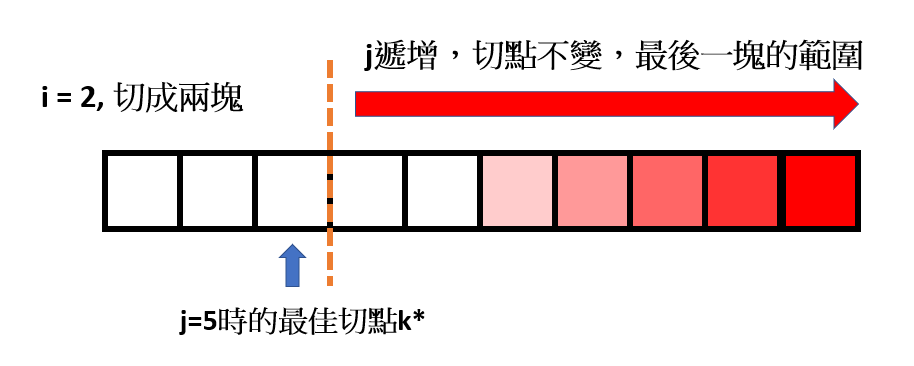
\includegraphics[scale=0.4]{./DP2/D_and_C_DP.png}}
		\caption{示意圖,人數變多時若切點$k$不往$k$大的方向前進,那最後一塊佔的比例將會越來越大,顏色越深代表越新加入。當$j$往箭頭方向增加時,最佳切點$k^*$同時也應該往箭頭方向前進。}
	\end{center}
\end{figure}

有了這個直覺後證明的方向就很清楚了,首先先將轉移式中的花費函數簡記,定義$C(k, j) = (\sum_{p = k + 1}^{p = j} \sum_{q = k + 1}^{q = j} u[p][q])$,可以發現$C(k, j)$其實是矩陣$u$中以$(k + 1, k + 1)$為左上角,$(j, j)$為右下角的子矩陣。

\begin{figure}[h!]
	\begin{center}
		\centerline{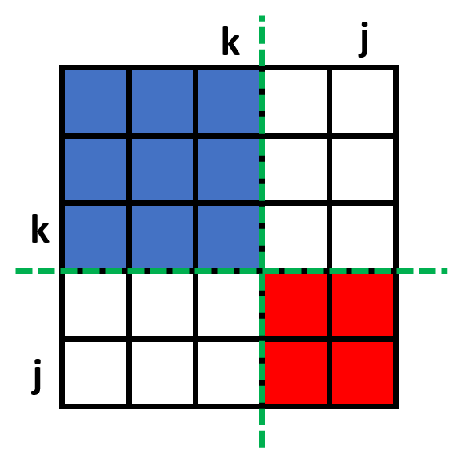
\includegraphics[scale=0.4]{./DP2/cost_function.png}}
		\caption{示意圖,$i$=2時選擇$k$為切點的花費,第一塊為左上塗色部分,第二塊為右下塗色部分。}
	\end{center}
\end{figure}
當$i$不變,$j$增加為$j + 1$時,轉移策略需要做哪些改變?首先,切點的選擇在最後面多出了切在$j$這個選項,而對於每個原先可選擇的切點k,則各自需要加入\textbf{這種切法下,這一塊的每個人$p$與第$j+1$人一起貢獻的花費$u[p][j + 1]$},也就是$\sum_{p = k + 1}^{p = j + 1} u[p][j + 1] + \sum_{p = k + 1}^{p = j + 1} u[j + 1][p]$,由於所有$u[i][j]$都非負,由上述式子極容易得證\textbf{$k$越小的切點,在人數增加時花費增加越多。($k$越小,$C(k, j + 1) - C(k, j)$越大)},畫成圖更容易理解,請參照圖5。

\begin{figure}[h!]
	\begin{center}
		\centerline{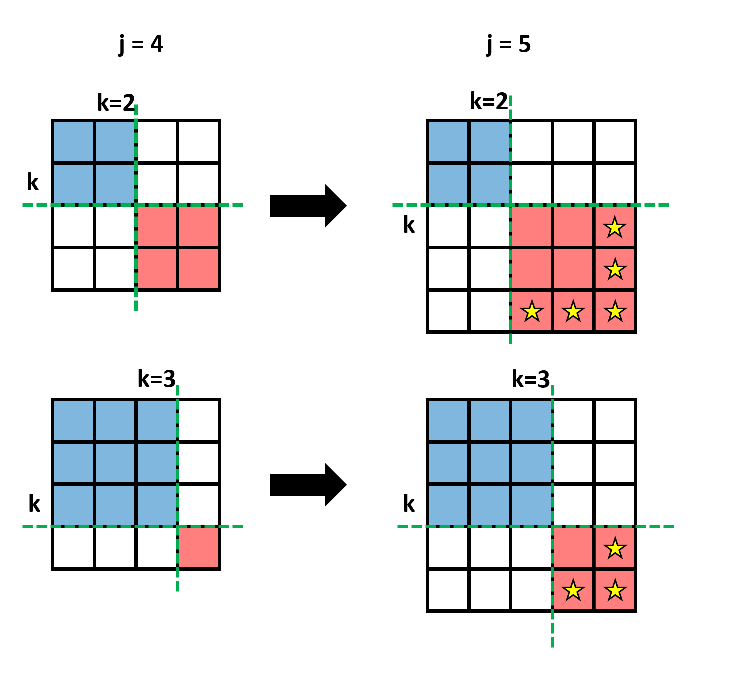
\includegraphics[scale=0.4]{./DP2/cost_change.png}}
		\caption{$i$=2, $j$=4變動到$j$=5時, 當$j$由4變動為5時,選擇切點$k$=2和$k$=3的cost變化,標註星星處為變動值。可看出$k$較大者增加的部分完全被$k$較小者包含。}
	\end{center}
\end{figure}

由此可知,\textbf{若一個切點$k$比最佳切點位置$k^*$要小,它的總花費原本就比切在$k^*$更大,在人數增加時,花費漲幅又比切在$k^*$更大},自然在往後都不可能成為最佳切點,也就是說,\textbf{有可能取代原本最佳切點$k^*$,成為新最佳解的切法$k$必定大於$k^*$},再換句話說,當人數增加時,最佳切點總是往$k$大的方向跑,就得證了想要的性質。

證出了這個性質後,優化的方式反而相對簡單。令$k_1, k_2, ..., k_N$分別為$dp[i][1], dp[i][2], ..., dp[i][N]$發生最佳解的切點,那麼\textbf{這個數列必須遞增}(非嚴格)。請參照圖6,此時若將$dp[i]$這個陣列中每個$dp[i][j]$都畫一個箭頭指向它在$dp[i - 1]$產生最佳解的位置,也就是$dp[i - 1][k_j]$,很明顯的,這些箭頭要不就不相交,要不就交於端點,絕不可能在中途交叉,這是由於\textbf{兩箭頭在中途交叉,代表起點較後面的箭頭指向較前面的點,這與前面證出的性質矛盾}。

\begin{figure}[h]
	\begin{center}
		\centerline{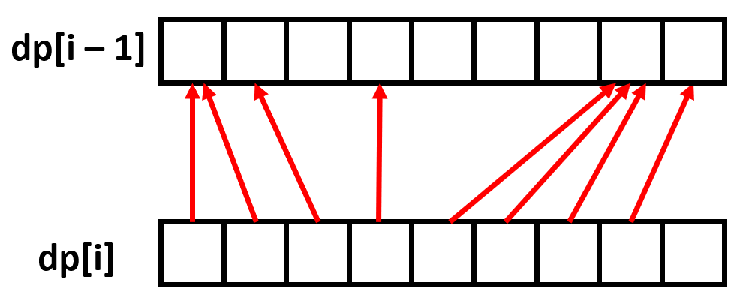
\includegraphics[scale=0.4]{./DP2/arrow.png}}
		\caption{每個$dp[i][j]$指向$k_j$,即枚舉$dp[i - 1][k] + C(k, j)$時產生最佳解的位置,應該形成一些無交叉的箭頭。請注意這只是示意圖,實際上$j < i$的狀態都是不存在的。}
	\end{center}
\end{figure}

但這些箭頭無交叉又如何呢?找出一個箭頭必須花$\Ord(N)$的時間把$dp[i - 1]$全都檢查過一次,算出全部箭頭在最差情況下仍然是$\Ord(N^2)$,但是這是完全無視性質的算法,身為一個學演算法的人,看到這些無交叉的箭頭應該很直覺會想先找出中間那一個!請參照圖7,\textbf{一旦知道中間那一個箭頭指向哪裡,那麼它左右兩邊最佳解有可能發生的區域不就被切成兩段了嗎?}

\begin{figure}[h]
	\begin{center}
		\centerline{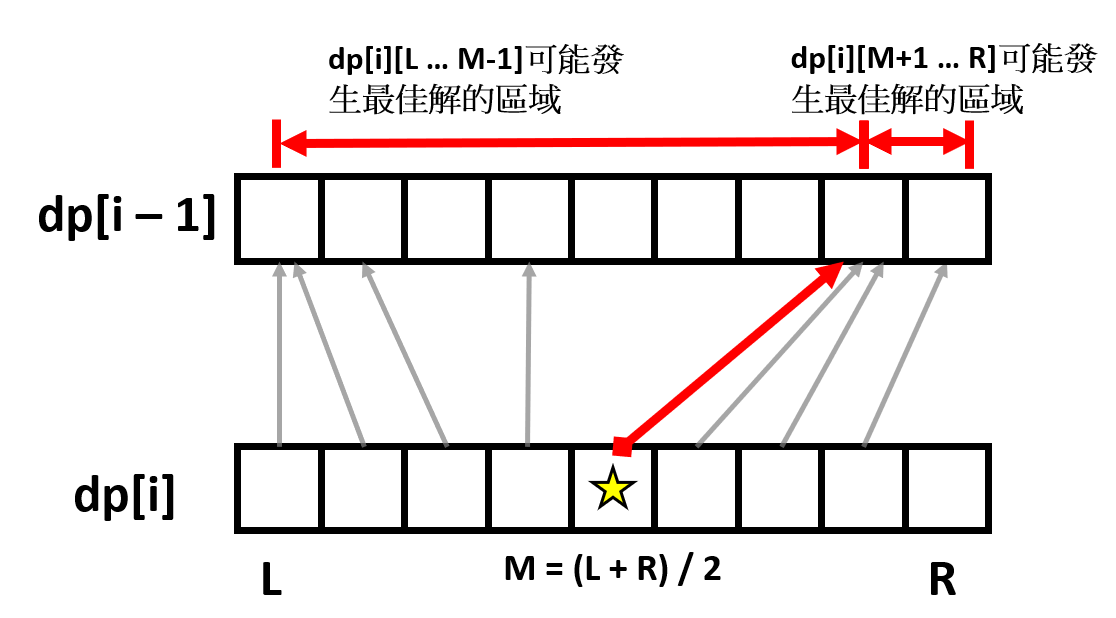
\includegraphics[scale=0.4]{./DP2/arrow_cut.png}}
		\caption{一旦找出中間的箭頭後,最佳解發生的區域就被切成兩段。}
	\end{center}
\end{figure}

顯然左邊的箭頭只會指向最佳解發生區域的左半塊,右邊的箭頭則對上右半塊,用分治的想法,把$dp[i]$陣列左右兩段分別遞迴求解。就得到了如下的演算法:
\begin{enumerate}
    \item 定義$Solve(i, L, R, opt\_L, opt\_R):=$ 計算$dp[i][L\mbox{ ... }R]$, 已知其中任一格的最佳解皆只能出現在$dp[i - 1][opt\_L\mbox{ ... }opt\_R]$。
    \item 令$M=\floor{\frac{L+R}{2}}$,暴力枚舉所有切點$k \in [opt\_L, opt\_R]$,求出$dp[i][M]$的最佳切點$k_M$。
    \item 最佳解區域被分成了兩塊,因此遞迴地呼叫$Solve(i, L, M-1, opt\_L, k_M)$與$Solve(i, M+1, R, k_M, opt\_R)$,將左右兩邊計算完成。
\end{enumerate}
此遞迴過程每次都將$dp[i]$陣列減半,顯然會得到一棵高度$\Ord(\log N)$的遞迴樹,同一層的每個節點的最佳解區域長度加起來只有$\Ord(N)$這麼長,每一個節點做的事是掃過一次自己的可行解區域,把中間的箭頭暴力找出來,因此同一層所有節點花的時間加起來是$\Ord(N)$的,總時間$\Ord(N \log N)$。

有了這個做法後,由$dp[i - 1]$整個陣列轉移到$dp[i]$整個陣列只需花$\Ord(N \log N)$的時間,算出整個$dp$表格只需花$\Ord(KN \log N)$,即可順利解出此題。最後附上code和演算法的回顧供讀者思考。

\begin{lstlisting}[caption=Ciel and Gondolas的程式碼,這題時限卡很緊,必須使用getchar。]

/* u: 花費矩陣的二維前綴和,請注意此題可用滾動壓低dp陣列使用的記憶體,請讀者自行思考如何實作  */
int N, K, u[MAX_N][MAX_N], dp[MAX_K][MAX_N];

inline int get_cost(int k, int i) {
	/* 利用2D前綴和計算C(k, j) */
	return (u[i][i] - u[i][k] - u[k][i] + u[k][k]) / 2;
}

/* D&C DP optimization的主體,計算dp[i][l ... r], 已知其中任一格的最佳解只會發生在dp[i - 1][opt_l ... opt_r] */
void solve(int i, int l, int r, int opt_l, int opt_r) {
	/* best紀錄目前的最佳解, where紀錄最佳解發生的切點 */
	int m = (l + r) / 2, best = INF, where = -1;

	/* 暴力枚舉可能的切點k,求出dp[i][m] */
	for (int k = opt_l; k <= min(m - 1, opt_r); k++) {
		int relax = dp[i - 1][k] + get_cost(k, m);
		if (relax < best) {
			best = relax;
			where = k;
		}
	}
	dp[i][m] = best;

	/* 知道dp[i][m]的最佳切點where後,最佳解區域就被切成了兩塊,dp[l .. m-1]對應左半邊,dp[m+1 ... r]對應右半邊。遞迴求解時須注意左右兩塊是否為空。 */
	if (l < m) solve(i, l, m - 1, opt_l, where);
	if (m < r) solve(i, m + 1, r, where, opt_r);
}

int main() {
	/* 輸入並建造2D前綴和,輸入必須使用getchar才夠快, */
	scanf("%d %d", &N, &K);
	for (int i = 1; i <= N; i++) {
		for (int j = 1; j <= N; j++) {
			char ch;
			do {
				ch = getchar();
			} while (ch < '0' || ch > '9');
			u[i][j] = u[i - 1][j] + u[i][j - 1] - u[i - 1][j - 1] + (ch - '0');
		}
	}

	/* dp計算主體就是把dp[i]從1到K算一遍,每次使用dp[i-1]去算dp[i]都是一次D&C。 */
	for (int j = 1; j <= N; j++) {
		dp[1][j] = get_cost(0, j);
	}
	for (int i = 2; i <= K; i++) {
		/* 請注意在題目給定條件下,所有j < i的dp[i][j]都是不存在的。 */
		solve(i, i, N, i - 1, N);
	}

	printf("%d\n", dp[K][N]);
}
\end{lstlisting}

小回顧:
\begin{enumerate}
\item 證出所有箭頭無交叉時,讀者有想過D\&C以外的方法嗎? 例如總是記住上一個箭頭發生的位置,這個方法在甚麼情況下會退化成$\Ord(N^2)$?
\item 為何在前面的分析寫說遞迴樹某一層是$\Ord(N)$而不是正好$N$?樹中同一層的兩節點間需要測試的最佳解區域有可能有交集嗎?這些交集會影響複雜度嗎?請試著用遞迴樹中的節點數量給出一個所有交集總長度的上界。
\item 如果將此問題改成容許空的切塊,也就是拿掉$q_i > 0$這個條件,請證明答案是否會改變,這樣改動後,轉移範圍會比較好找嗎?
\item 這個DP很明顯可以用滾動壓低記憶體,請讀者自行思考。
\item 如果稍微改變計算順序,以人數$j$為外層迴圈,塊數$i$為內層迴圈計算,那麼$dp[j - 1]$整個陣列轉移到$dp[j]$整個陣列的過程可說是證不出任何性質(這裡$dp[j]$陣列指的是$dp$表格的整個column $j$)。因為當人數$j$固定,塊數$i$變動成$i + 1$時,對於每個切點$k$,花費會由$dp[i - 1][k] + C(k, j)$變動為$dp[i][j] + C(k, j)$,\textbf{跟著$i$變動的是$dp[i][j]$這個函數}。花費函數$C(k, j)$可以看作是簡單的子矩陣和,容易證出各種性質,相較之下,我們對於$dp[i][j]$這個函數可說是一無所知,在它變動時根本無從下手。因此一旦改變了計算順序,想解開此問題的難度就會大幅提升。
\item 前面說過直覺上每塊應該切的越平均越好,但是直接greedy的想法肯定是錯的。假設有個greedy解猜測最佳轉移只有可能發生在$\floor{\frac{N}{K}}$或$\ceil{\frac{N}{K}}$兩種切法上,在研讀了花費函數的性質後,讀者能給出一個一眼就能知道greedy不對的反例嗎?
\end{enumerate}

進階DP章節到此結束,最後這一節主要目的是讓讀者欣賞藝術,所以不提供此優化的練習題,希望上述演算法和證明過程的想法 / 概念可以給讀者一些啟發。如果真的很想寫這種題目的話,將本章標題餵給google即可找到不少。

\subsection{練習題}
有些技巧其實不算太難想到,或是並沒有很精彩,但是比賽會出,筆者將它們蒐集在練習中。此處的問題非常雜亂,沒必要刻意在短時間將他們全部寫完,知道這種東西是能做的,日後遇到再來想即可。
\problembox{Convex Hull Trick}{經典問題}{
Convex Hull Trick是最常出現在比賽的進階DP技巧,在這本講義被歸類在幾何,請讀者在幾何篇章中學習。
}
\problembox{直線最大值}{經典問題}{
請嘗試在不維護Convex Hull的條件下解決此問題。\newline
給定平面上$N$條直線函數$f_i(x) = a_{i}x + b_i$和$Q$筆詢問,每次詢問給定一座標$x_j$,求$\max\{f_i(x_j) : i \in [1, N]\}$,假設$Q$與$N$同階,$\Ord(N \log N)$。\newline
$Hint: $試著將此問題跟D\&C DP優化用到的技巧連結在一起。
}
\problembox{Grouping}{AtCoder Regular Contest 067}{
    $Hint:$ 將解法的複雜度精準地列下來,不要每一步都高估,也許會收斂到比想像的更小。
}
\problembox{枚舉submask}{經典問題}{
試證明以下程式碼花費$\Ord(4^N)$的時間輸出$3^N$。\newline
$Hint: 3^N$ 在排列組合中代表甚麼?此問題也有代數證法。
}
\begin{lstlisting}[caption=待證明程式碼]
int ans = 0;
for (int m = 0; m < (1 << N); m++) {
    for (int s = 0; s < (1 << N); s++) {
        if ((m | s) == m) {
            /* s is submask of mask m in binary representation */
            ans++;
        }
    }
}
cout << ans << '\n';
\end{lstlisting}
\problembox{枚舉submask 2}{經典問題}{
    試證明對於每個i,下方程式進入for迴圈內的$j$的集合,與上方程式進入if內的$j$的集合完全相同。並證明此程式可在$\Ord(3^N)$時間內完成。
}
\begin{lstlisting}[caption=待證明程式碼]
int ans = 0;
for (int m = 0; m < (1 << N); m++) {
    for (int s = m; ; s = (s - 1) & m) {
        /* s is submask of mask m in binary representation */
        ans++;
        if (s == 0) break;
    }
}
cout << ans << '\n';
\end{lstlisting}
\problembox{Grouping}{AtCoder Educational DP Contest}{
這題和前面的Grouping不同,只是剛好同名。
}
\problembox{Sum Over Subset}{經典問題}{
請利用DP,在$\Ord(N \times 2^N)$時間內算出以下程式碼的dp陣列。\newline
$Hint:$ $\Ord(N \times 2^N)$個狀態,$\Ord(1)$轉移。
}
\begin{lstlisting}[caption=Sum Over Subset]
/* N, and a[0 ... (1 << N)-1] is input array */
for (int m = 0; m < (1 << N); m++) {
    for (int s = 0; s < (1 << N); s++) {
        if ((m | s) == m) {
            /* s is submask of m in binary representation */
            dp[m] += a[s]
        }
    }
}
cout << ans << '\n'
\end{lstlisting}
\problembox{Appropriate Team}{CF 1016G}{
$Hint:$ 這麼大的數能質因數分解嗎?
}
\problembox{Intense Heat}{CF 1003C}{
    請嘗試在$\Ord(N \log N)$時間內解決此問題。\newline
    $Hint:$ 將所有要枚舉的$(j, dp[j])$畫在平面上,$dp[i]$等同要求最大化通過$(j, dp[j])$與$(i, dp[i])$直線的斜率,最佳轉移是否一定出現在凸包上? 另外,此題有較難證明的$\Ord(N)$解。
}

\newpage
